\documentclass{beamer}
\usepackage[english]{babel}
\usepackage{geometry}
\usepackage[utf8]{inputenc}
\usepackage{colortbl}
\usepackage{listings}
\usepackage{adjustbox}
\usepackage{verbatim}
\usepackage{amsmath}
\usepackage{multirow}
\usepackage{tabularx}
\usepackage{tikz}
\usepackage[linewidth=1pt]{mdframed}
\usepackage[utf8]{inputenc}
\usepackage{listings}
\usepackage{color}

\definecolor{dkgreen}{rgb}{0,0.6,0}
\definecolor{gray}{rgb}{0.5,0.5,0.5}
\definecolor{mauve}{rgb}{0.58,0,0.82}

\usetheme{Madrid}
% \usecolortheme{Copenhagen}
\usenavigationsymbolstemplate{} % no navigation buttons
\usecolortheme{beaver}

% \setbeamercolor{block title}{bg=red!30,fg=black}


\title{TCP/IP in hardware }
\subtitle{- using SME}
\author{Mark Jan Jacobi \& Jan Meznik}
\institute{University of Copenhagen}
\date{\today}


\begin{document}

\frame{\titlepage}

\section{Introduction}
\begin{frame}
  \frametitle{Background and Motivation}

  Dedicated hardware needs to transmit data in real time, but OS network
  stacks are usually not enough!

  Dedicated Network cards are not perfect either:
  \begin{columns}

 \begin{column}{0.7\textwidth}
  \begin{alertblock}{Weaknesses of network cards}
    \begin{itemize}
      \item Only basic programmability
      \item Incompatible APIs
      \item Licensed VHDL code blobs
      \item Seldom swap-able
      \item \textbf{Price!}
    \end{itemize}
  \end{alertblock}
  \end{column}

  \begin{column}{0.3\textwidth}
    \begin{figure}
    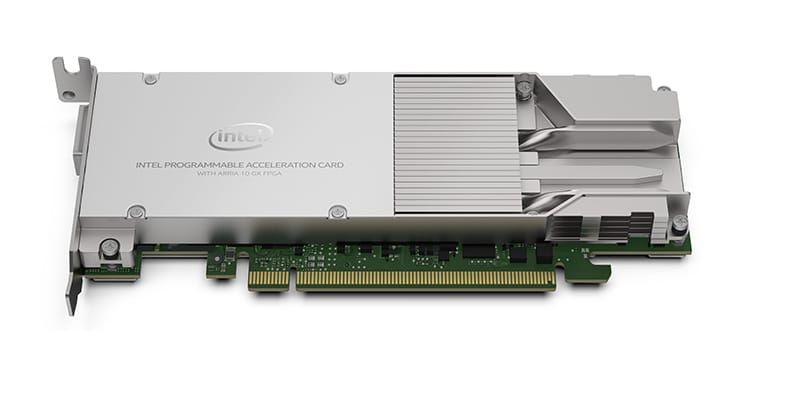
\includegraphics[scale=0.15,angle=270]{intel_fpga_nic.jpg}
    \caption{An Intel FPGA NIC}
    \end{figure}
  \end{column}

\end{columns}


\end{frame}
\begin{frame}
\begin{center}
  \textbf{A performant, efficient, and flexible network stack in FPGA!}
\end{center}

\begin{block}{How?    Using SME!}
  \begin{itemize}
    \item Easy \& intuitive hardware modelling
    \item Implicit clock
    \item Built-in simulation utilities
    \item VHDL code generation
    \item Verification by comparing VHDL signals with C\# simulation
  \end{itemize}
\end{block}

\end{frame}

\begin{frame}
  \frametitle{SME and FPGA}

  Skip this if SME has been covered
\end{frame}

\begin{frame}
  \frametitle{Internet Protocol Suite (TCP/IP)}
\begin{columns}

 \begin{column}{0.3\textwidth}
  \begin{center}
  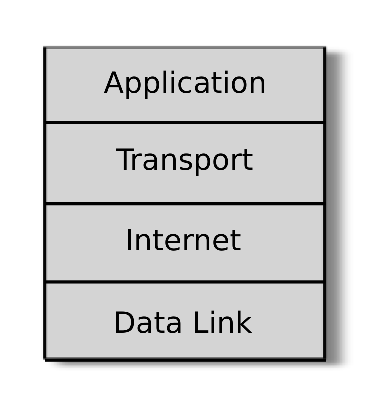
\includegraphics[scale=0.42]{tcpip_stack}
  \end{center}
  \end{column}

  \begin{column}{0.5\textwidth}
    \begin{itemize}
      \item<1->[Application] FTP, DHCP, SSH, etc.
      \item<2->[Transport] TCP, UDP, DCCP, etc.
      \item<3->[Internet] IPv4, IPv6, {\color{red} ICMP}, etc.
      \item<4->[Data Link] ARP, MAC (Ethernet, Wi-Fi), etc.
    \end{itemize}
  \end{column}
\end{columns}

\end{frame}




\section{Implementation}
\begin{frame}
  \frametitle{Architecture}
  \begin{center}
    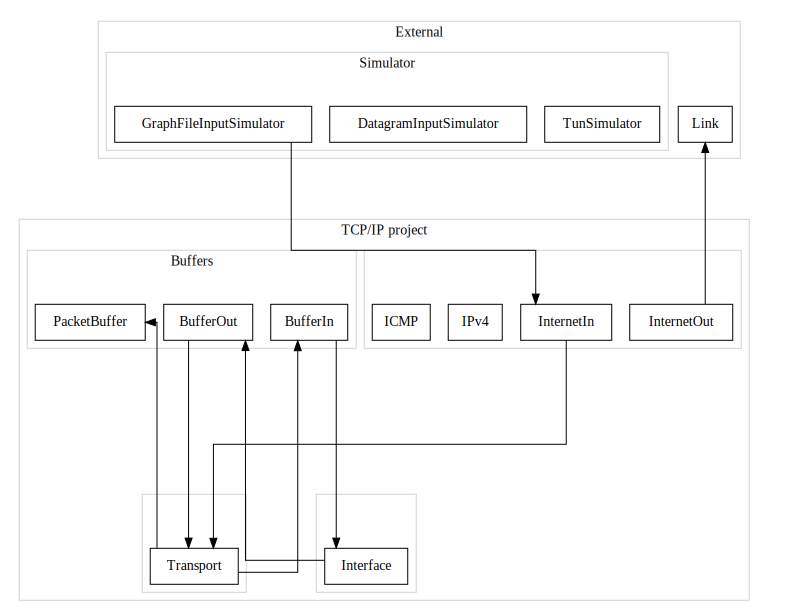
\includegraphics[scale=0.5]{graph}
  \end{center}


\end{frame}

\section{Challenges}
\begin{frame}[fragile]
  \frametitle{Challenges}

\begin{columns}
\begin{column}{0.5\textwidth}
\begin{itemize}
  \item<1-> Clock-delays and congestion
  \item<2-> Limited subset of programming language utilities
  \item<3-> Data de-multiplexing
  \item<4-> Limited (fast) memory
  \item<5-> Information sharing is by design hard in SME
\end{itemize}
\end{column}
\begin{column}{0.5\textwidth}
\includegraphics<1>[scale=0.5]{congest.eps}

\begin{overlayarea}{\linewidth}{3cm}
  \begin{onlyenv}<2>
  \begin{lstlisting}[language=c,frame=single]
// These are not allowed
O.M = new Func<int>(() => 
{ return 42; });

void Method(ref int x) {}

int* p1 = &x;
  \end{lstlisting}
  \end{onlyenv}
\end{overlayarea}  

\begin{onlyenv}<3>
\textbf{Packets up to 65,535 bytes!}
\end{onlyenv}
%\includegraphics<2>{B}
%\includegraphics<3>{C}
\end{column}
\end{columns}

\end{frame}

\section{Questions}
\begin{frame}
  \frametitle{Questions}
  \begin{center}
    ?
  \end{center}
\end{frame}


\end{document}



